\section{Auswertung}
\label{sec:Auswertung}

\subsection{Verifizierung der Funktionsweise eines Lock-In-Verstärkers}
\label{subsec:Verifizierung}
Die Spannungen werden für 7 Phasenverschiebungen in 60° Abständen aufgenommen.
Die entsprechenden Bilder des Oszilloskop ohne Rauschen sind in \autoref{fig:ohne} zu finden, die mit in \autoref{fig:mit}.
Die aufgenommenen Messwerte für die Untersuchung mit und ohne Noise Generator sind in \autoref{tab:data_ohne_mit} zu sehen.
Für beide Messvorgänge werden die Werte in Diagrammen veranschaulicht (siehe \autoref{fig:versuch_1_cosinus}) und mithilfe von python eine Ausgleichskurve nach Gleichung \eqref{eqn:Kosinus} bestimmt.
Die zu ermittelnde Gleichung lautet:
\begin{equation*}
  U = a * \cos(\phi)
\end{equation*}
Durch die Ausgleichsrechnung folgt:
\begin{align*}
  \text{ohne Noise Generator:}&  &a_\text{ohne} &= \SI{17 \pm 4}{\volt}, \\
  \text{mit Noise Generator:}&   &a_\text{mit}  &= \SI{10.7 \pm 2.9}{\volt}.
\end{align*}
Nach Gleichung \eqref{eqn:U_out} gilt für $a = \sfrac{2 \cdot U_0}{\pi}$, somit ergeben sich für $U_0$ folgende Werte:
\begin{align*}
  \text{ohne Noise Generator:}&  &U_{0,\text{ohne}} &= \SI{26.70 \pm 16.80}{\volt}, \\
  \text{mit Noise Generator:}&   &U_{0,\text{mit}}  &= \SI{ 6.28 \pm 4.56}{\volt}.
\end{align*}

\begin{figure}
  \label{fig:ohne}
  \begin{subfigure}{0.48\textwidth}
      \centering
      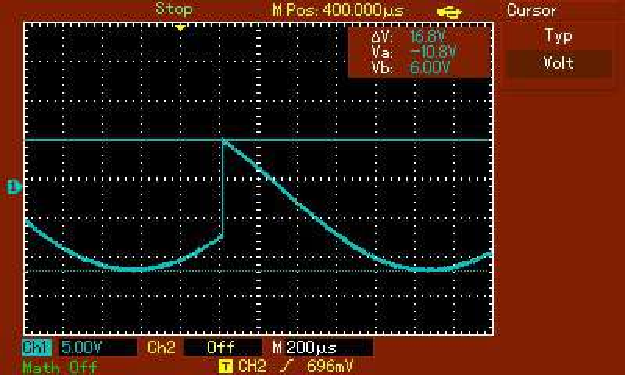
\includegraphics[height=5cm]{content/abbildungen/ohne/0.pdf}
      \caption{Spannung bei $\phi = 0°$ ohne Rauschen.}
  \end{subfigure}
\hfill 
  \begin{subfigure}{0.48\textwidth}
      \centering
      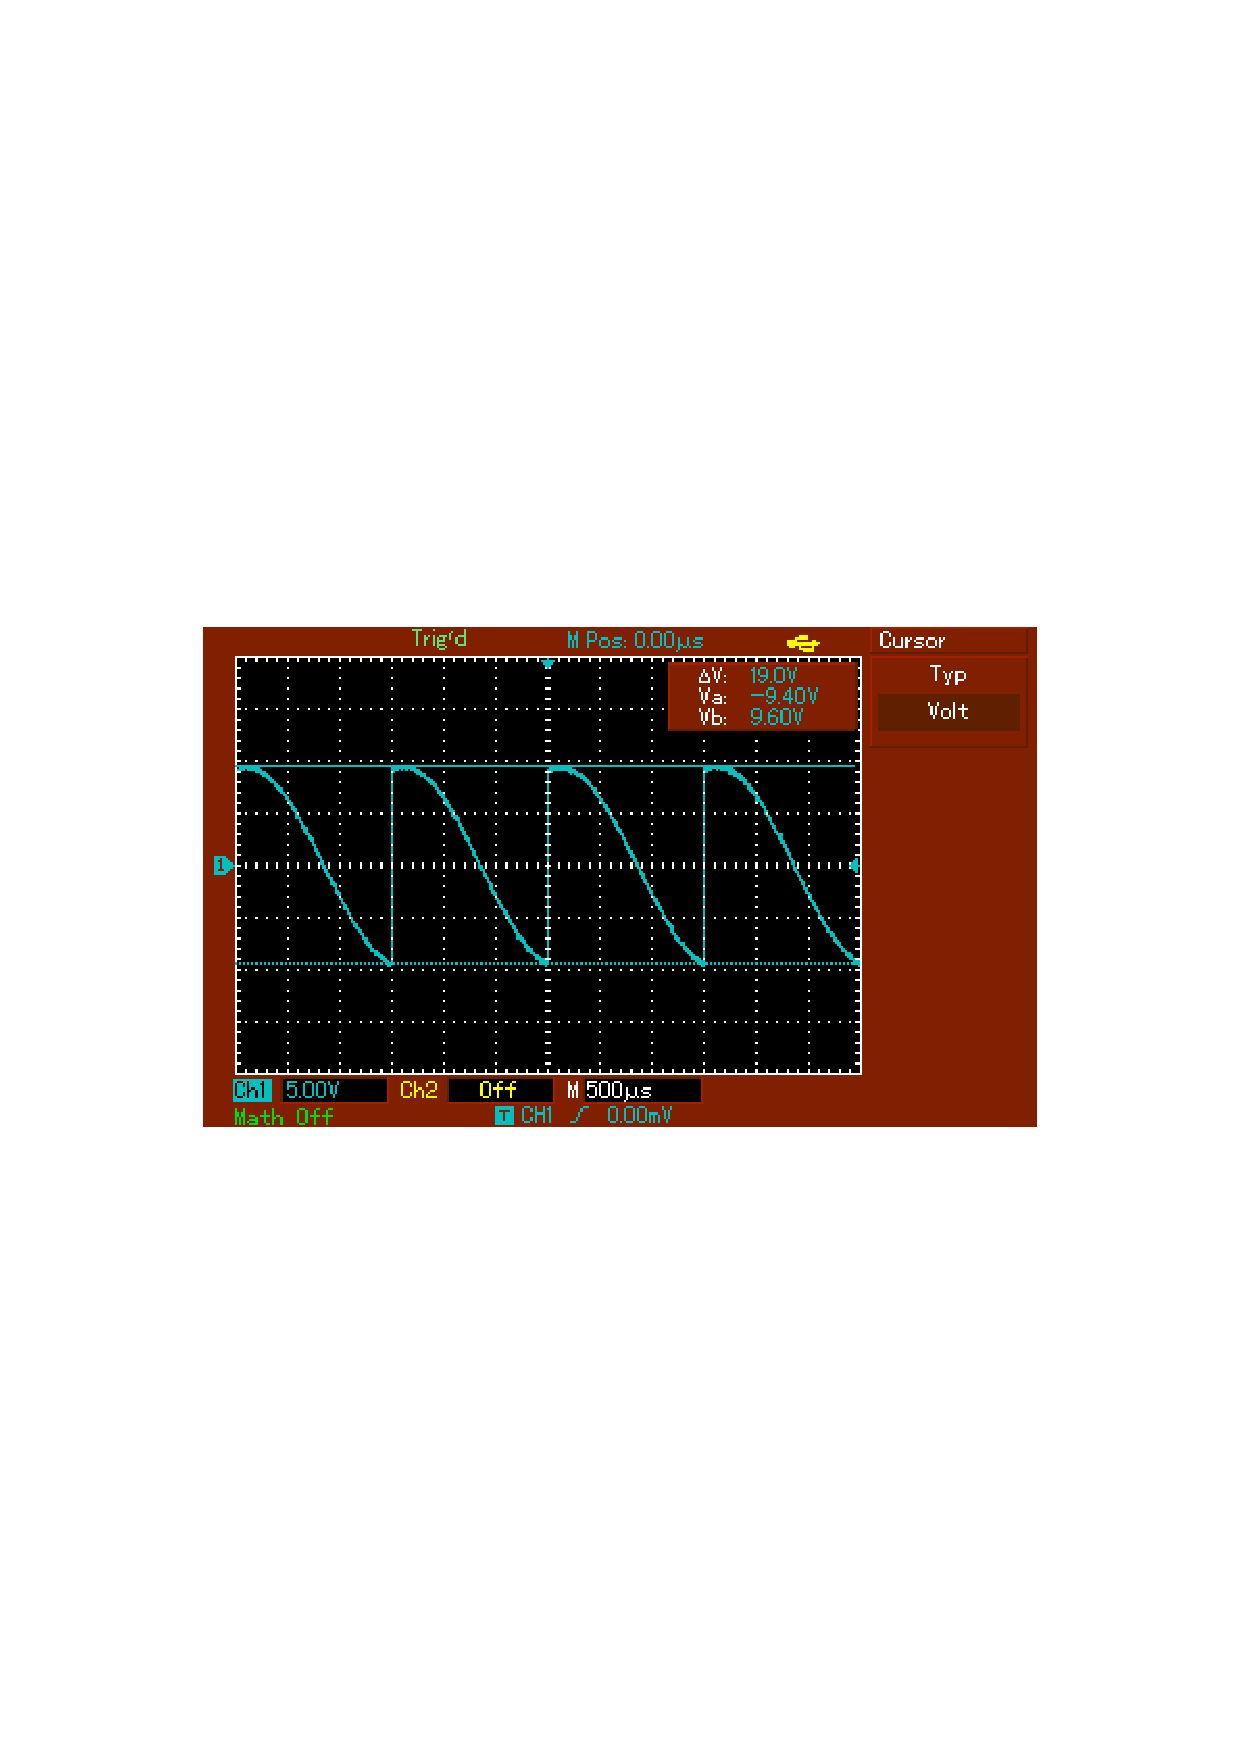
\includegraphics[height=5cm]{content/abbildungen/ohne/60.pdf}
      \caption{Spannung bei $\phi = 60°$ ohne Rauschen.}
  \end{subfigure}
\hfill 
  \begin{subfigure}{0.48\textwidth}
      \centering
      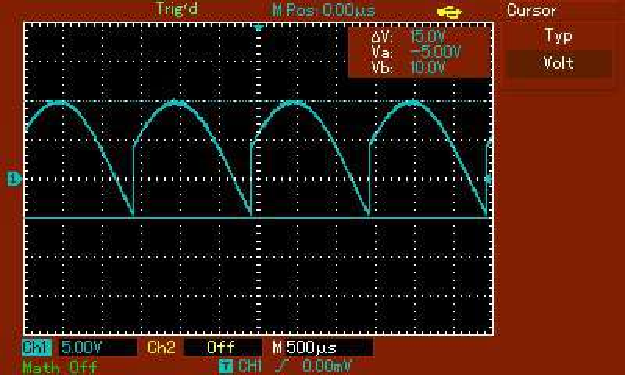
\includegraphics[height=5cm]{content/abbildungen/ohne/120.pdf}
      \caption{Spannung bei $\phi = 120°$ ohne Rauschen.}
  \end{subfigure}
\hfill 
  \begin{subfigure}{0.48\textwidth}
      \centering
      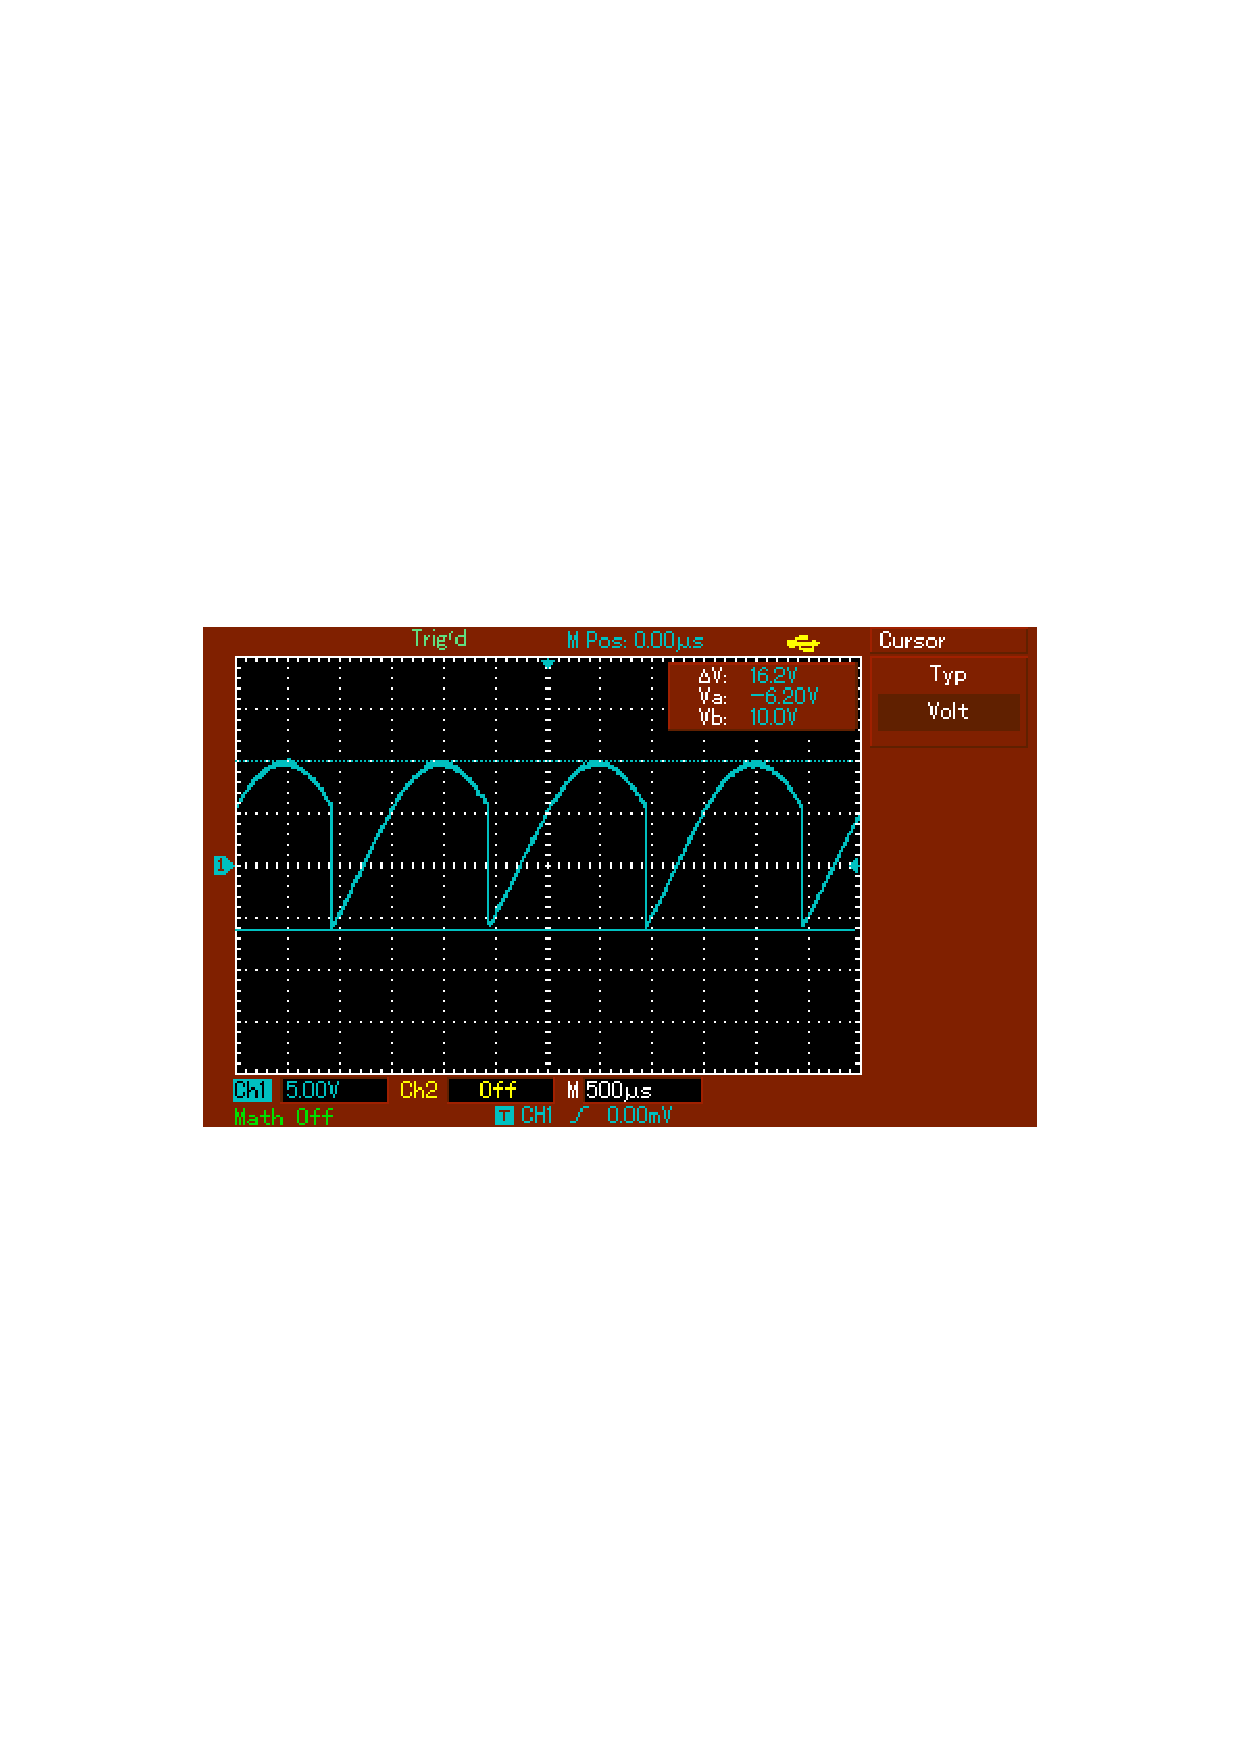
\includegraphics[height=5cm]{content/abbildungen/ohne/180.pdf}
      \caption{Spannung bei $\phi = 180°$ ohne Rauschen.}
  \end{subfigure}
\hfill 
  \begin{subfigure}{0.48\textwidth}
      \centering
      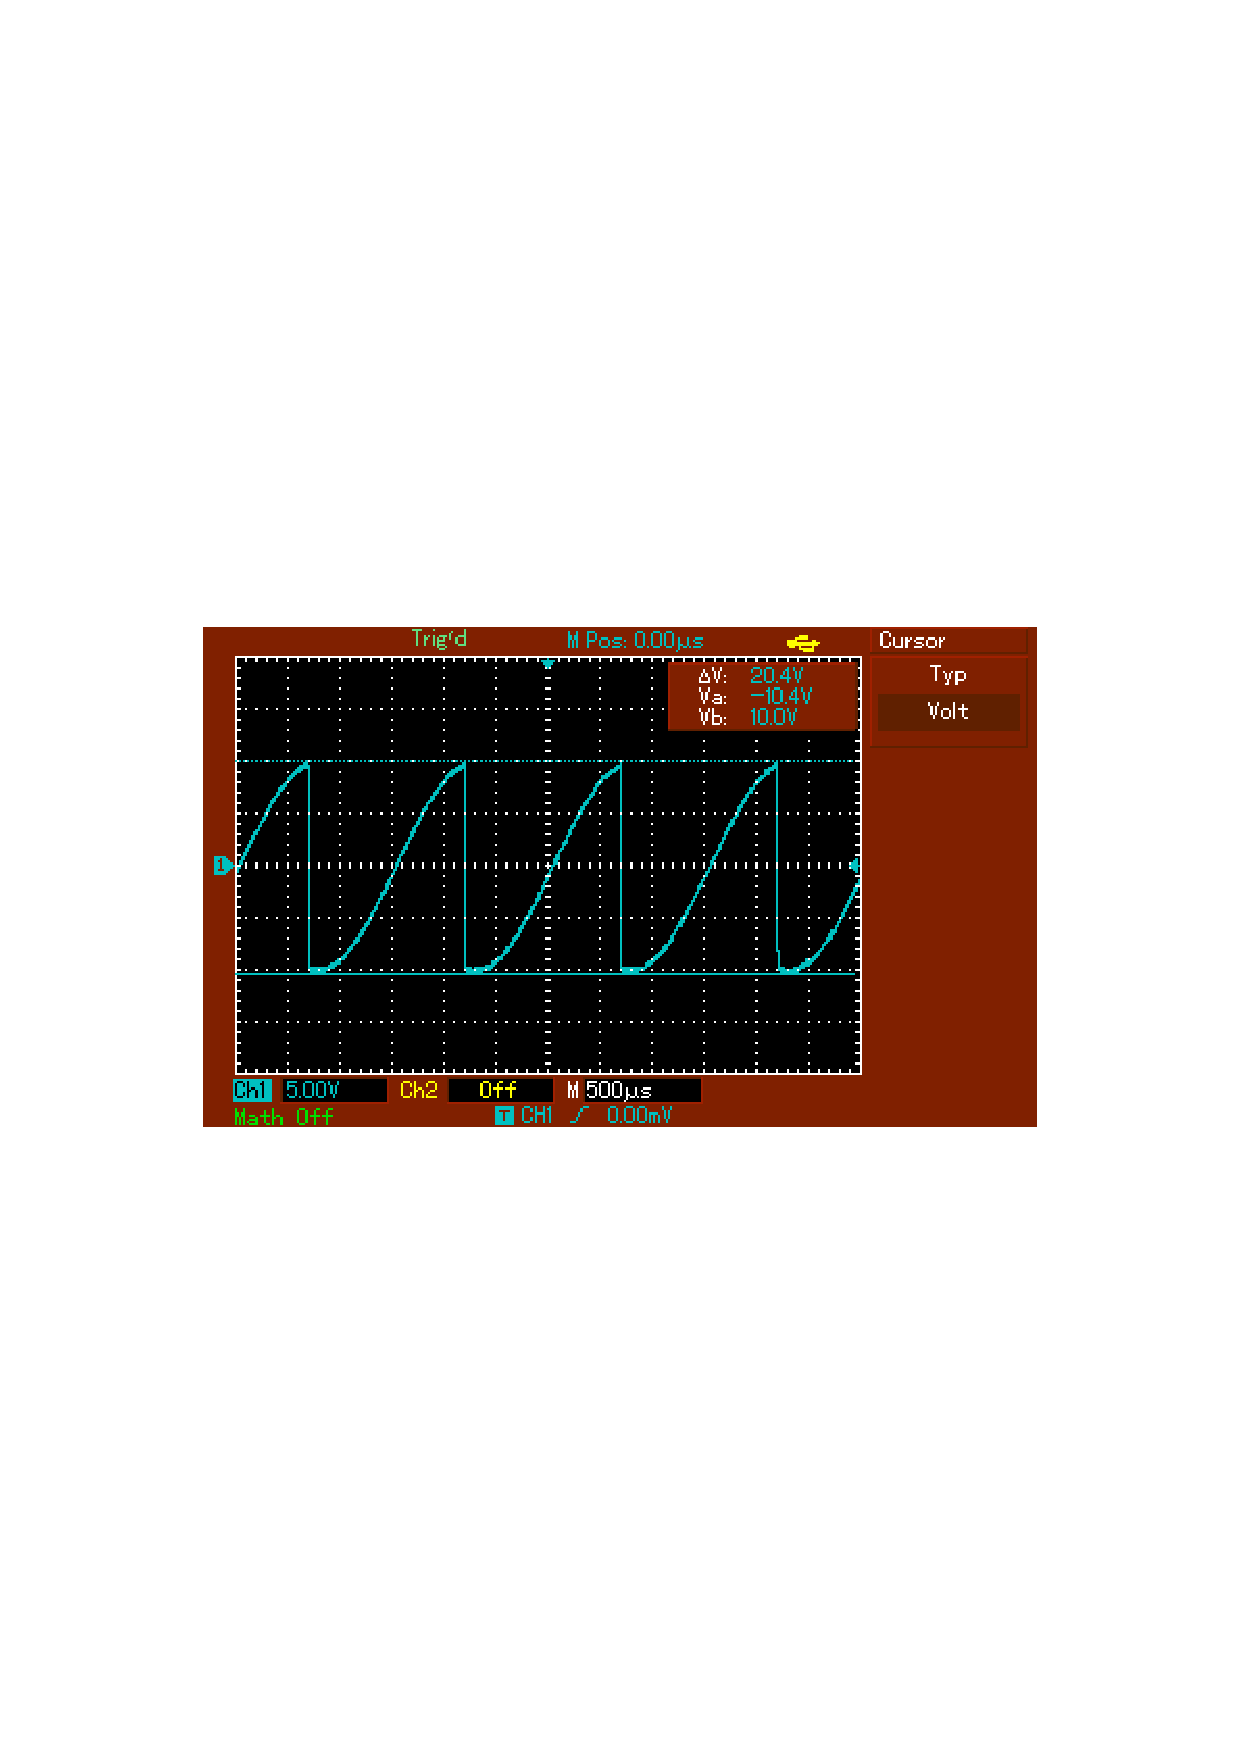
\includegraphics[height=5cm]{content/abbildungen/ohne/240.pdf}
      \caption{Spannung bei $\phi = 240°$ ohne Rauschen.}
      \end{subfigure}
\hfill 
  \begin{subfigure}{0.48\textwidth}
      \centering
      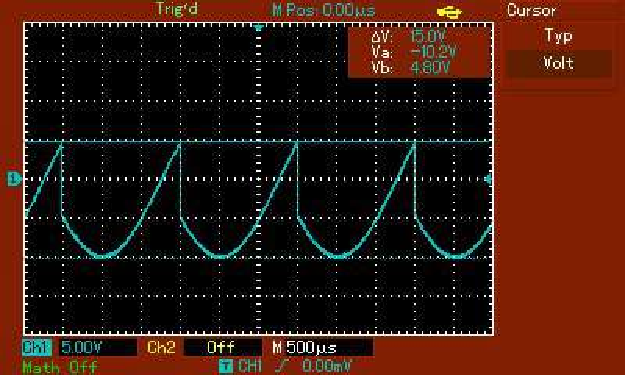
\includegraphics[height=5cm]{content/abbildungen/ohne/300.pdf}
      \caption{Spannung bei $\phi = 300°$ ohne Rauschen.}
      \end{subfigure}
\hfill 
  \begin{subfigure}{0.48\textwidth}
      \centering
      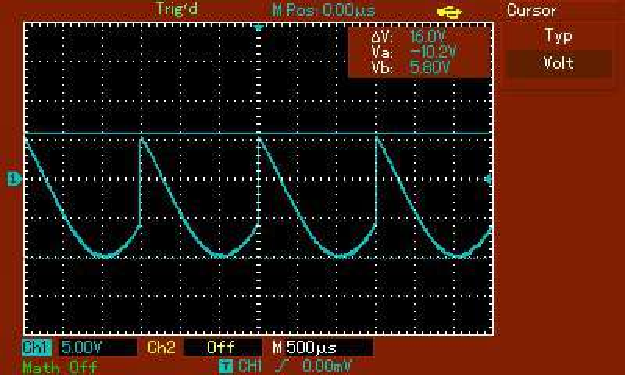
\includegraphics[height=5cm]{content/abbildungen/ohne/360.pdf}
      \caption{Spannung bei $\phi = 360°$ ohne Rauschen.}
      \end{subfigure}
\caption{Die Spannungen bei verschiedenen Phasenverschiebungen $\phi$ ohne Noise Generator.}
\end{figure}

\begin{figure}
  \label{fig:mit}
  \begin{subfigure}{0.48\textwidth}
      \centering
      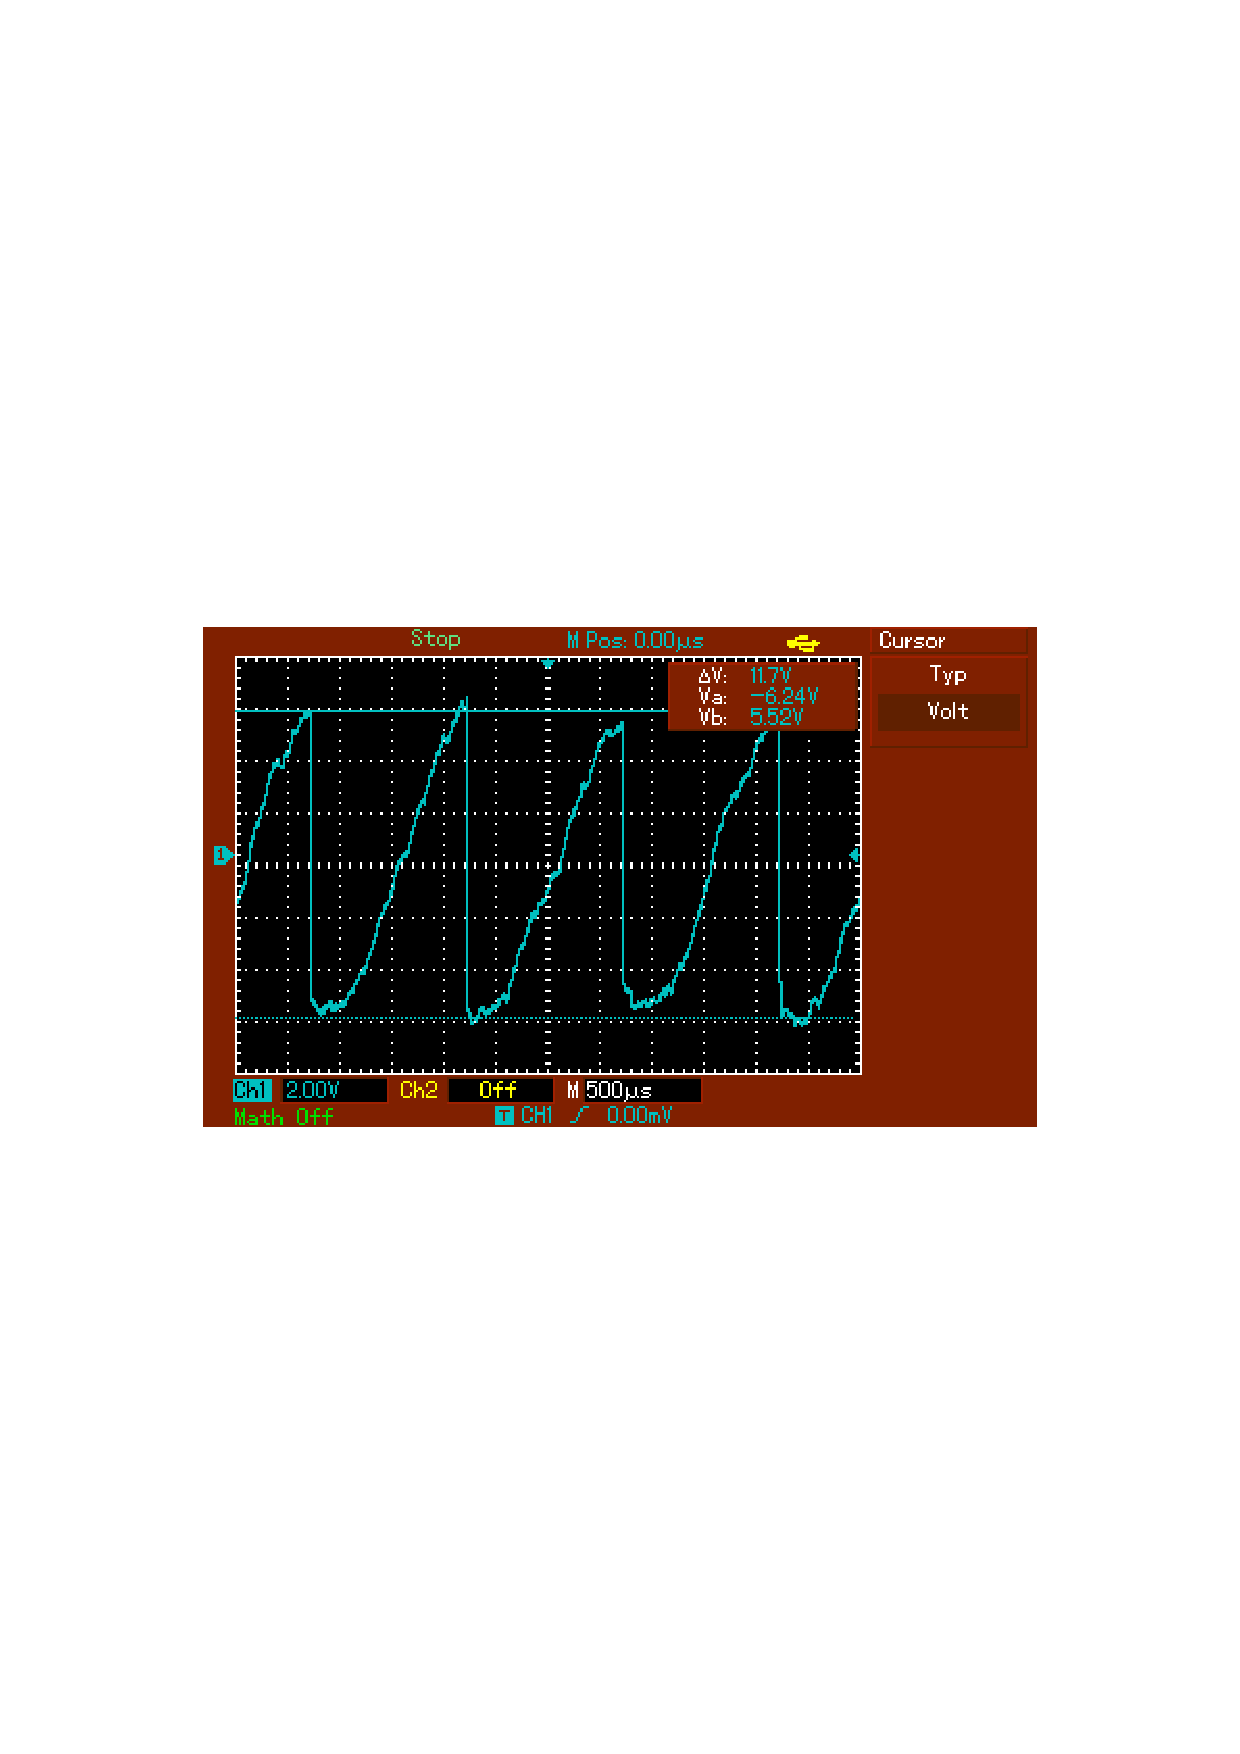
\includegraphics[height=5cm]{content/abbildungen/mit/0.pdf}
      \caption{Spannung bei $\phi = 0°$ mit Rauschen.}
  \end{subfigure}
\hfill 
  \begin{subfigure}{0.48\textwidth}
      \centering
      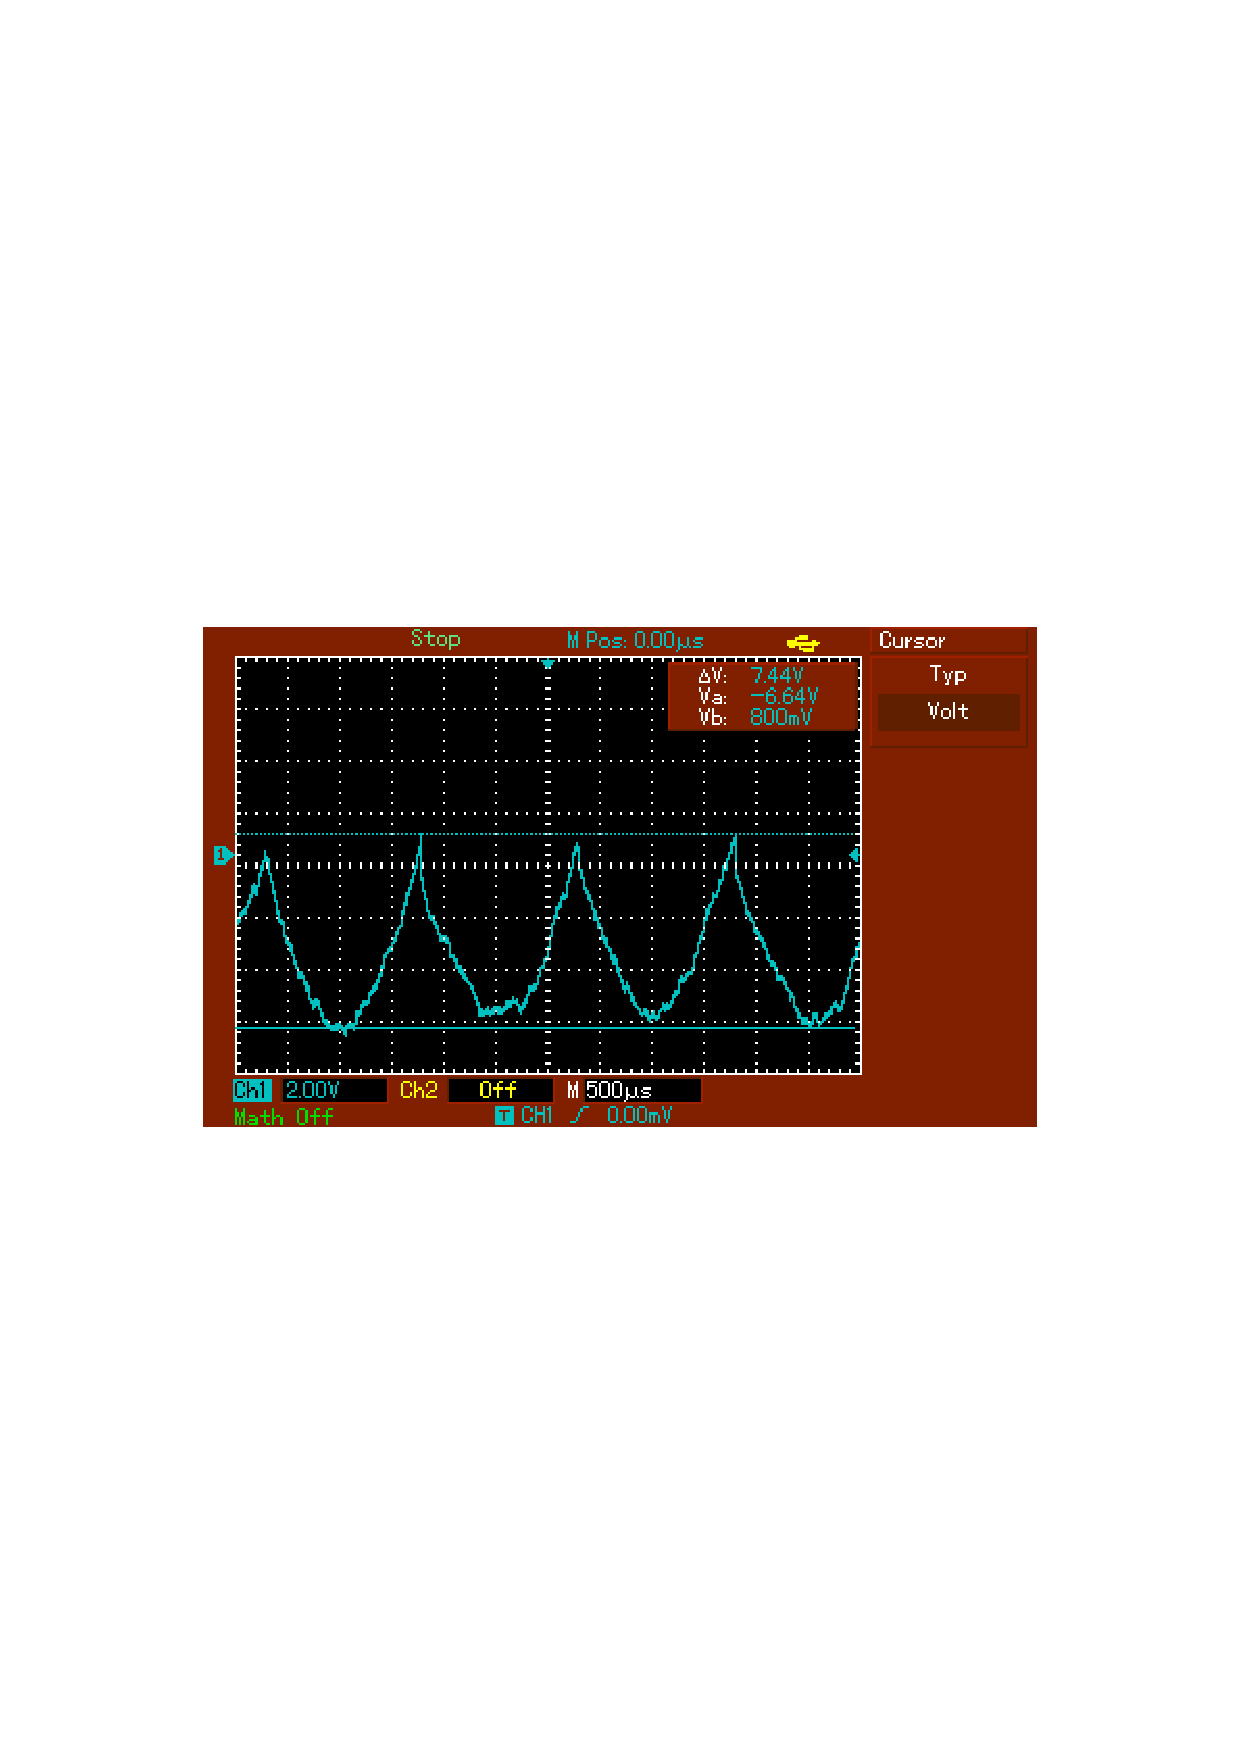
\includegraphics[height=5cm]{content/abbildungen/mit/60.pdf}
      \caption{Spannung bei $\phi = 60°$ mit Rauschen.}
  \end{subfigure}
\hfill 
  \begin{subfigure}{0.48\textwidth}
      \centering
      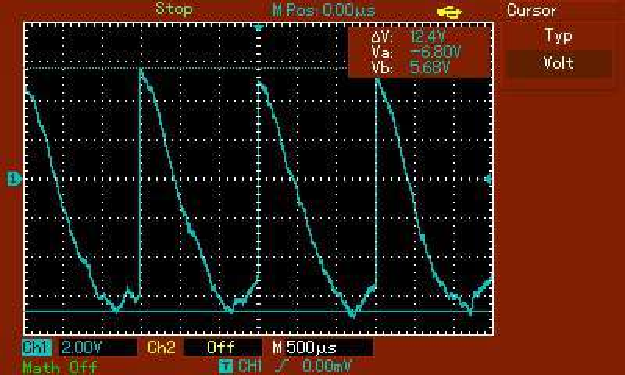
\includegraphics[height=5cm]{content/abbildungen/mit/120.pdf}
      \caption{Spannung bei $\phi = 120°$ mit Rauschen.}
  \end{subfigure}
\hfill 
  \begin{subfigure}{0.48\textwidth}
      \centering
      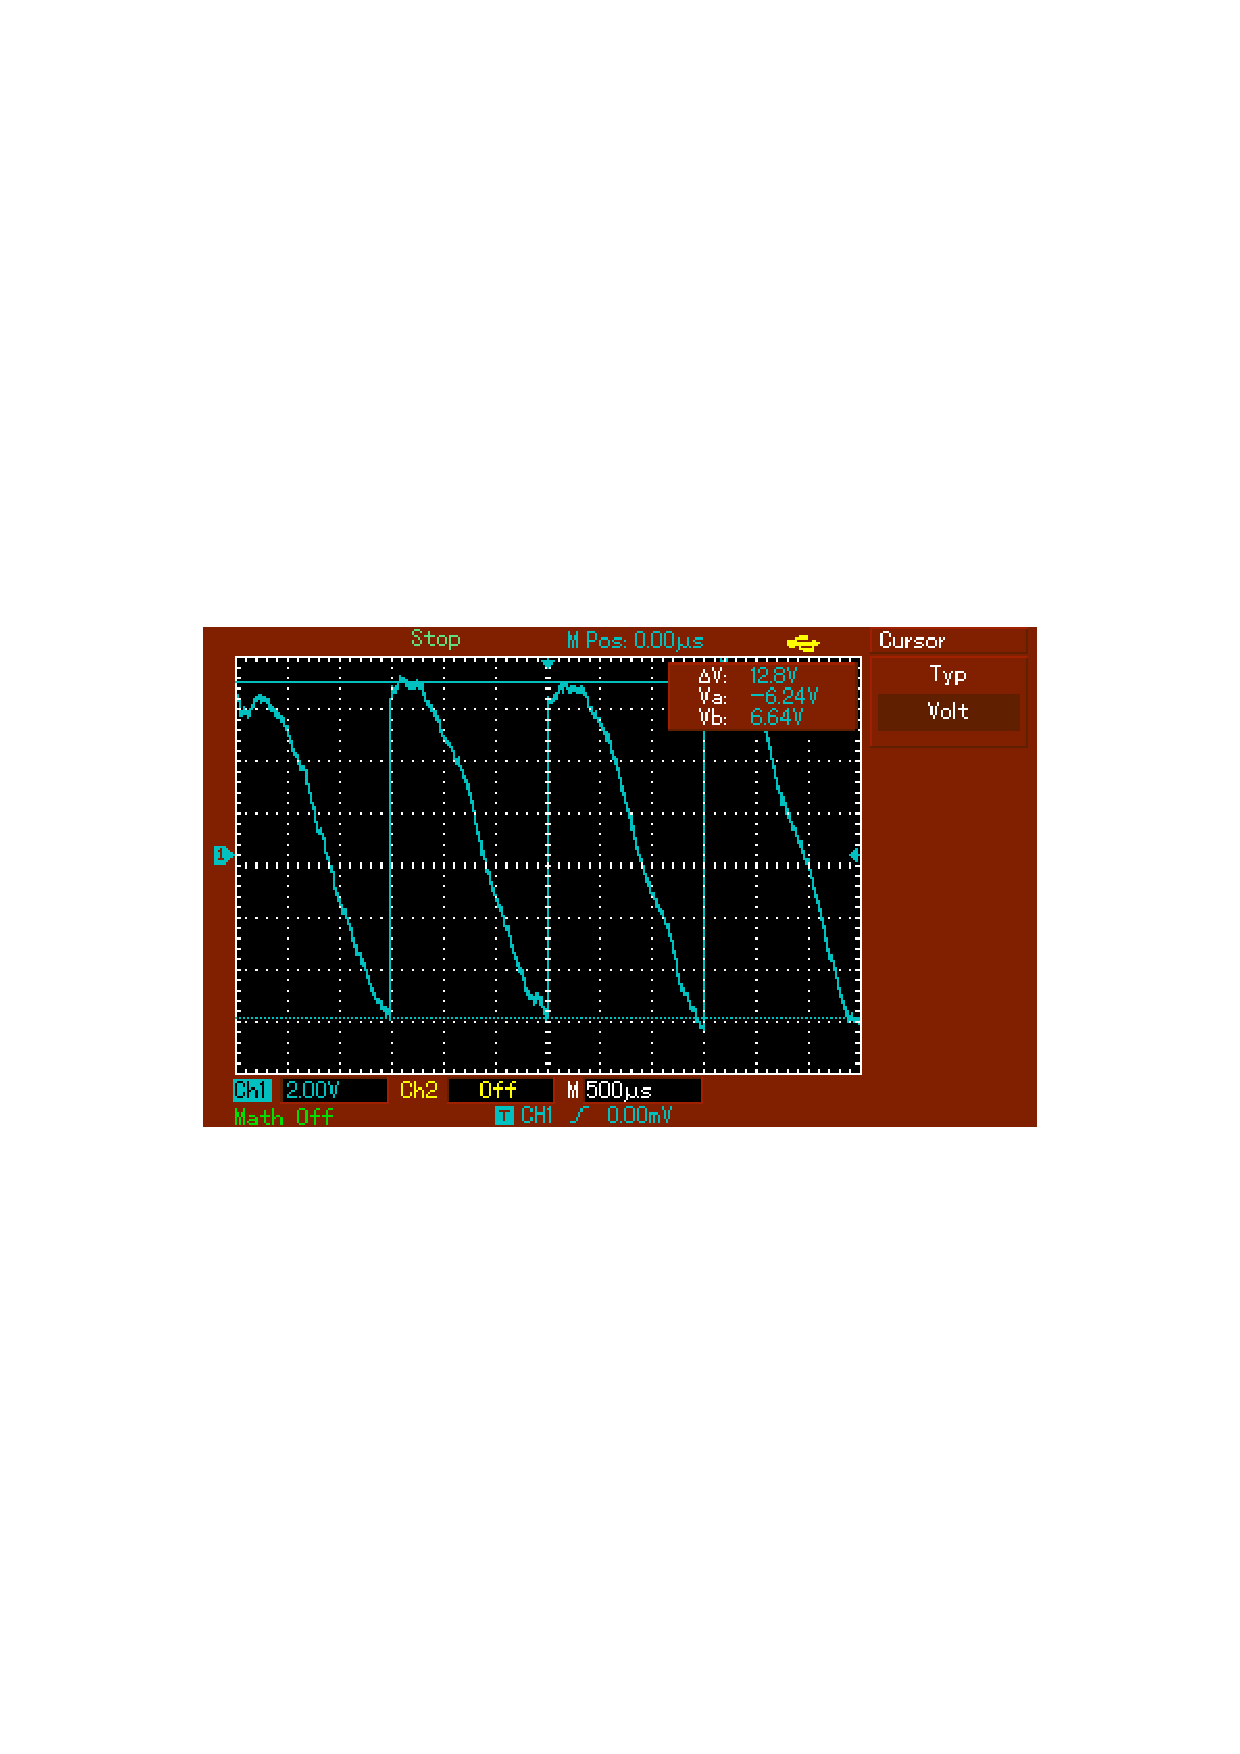
\includegraphics[height=5cm]{content/abbildungen/mit/180.pdf}
      \caption{Spannung bei $\phi = 180°$ mit Rauschen.}
  \end{subfigure}
\hfill 
  \begin{subfigure}{0.48\textwidth}
      \centering
      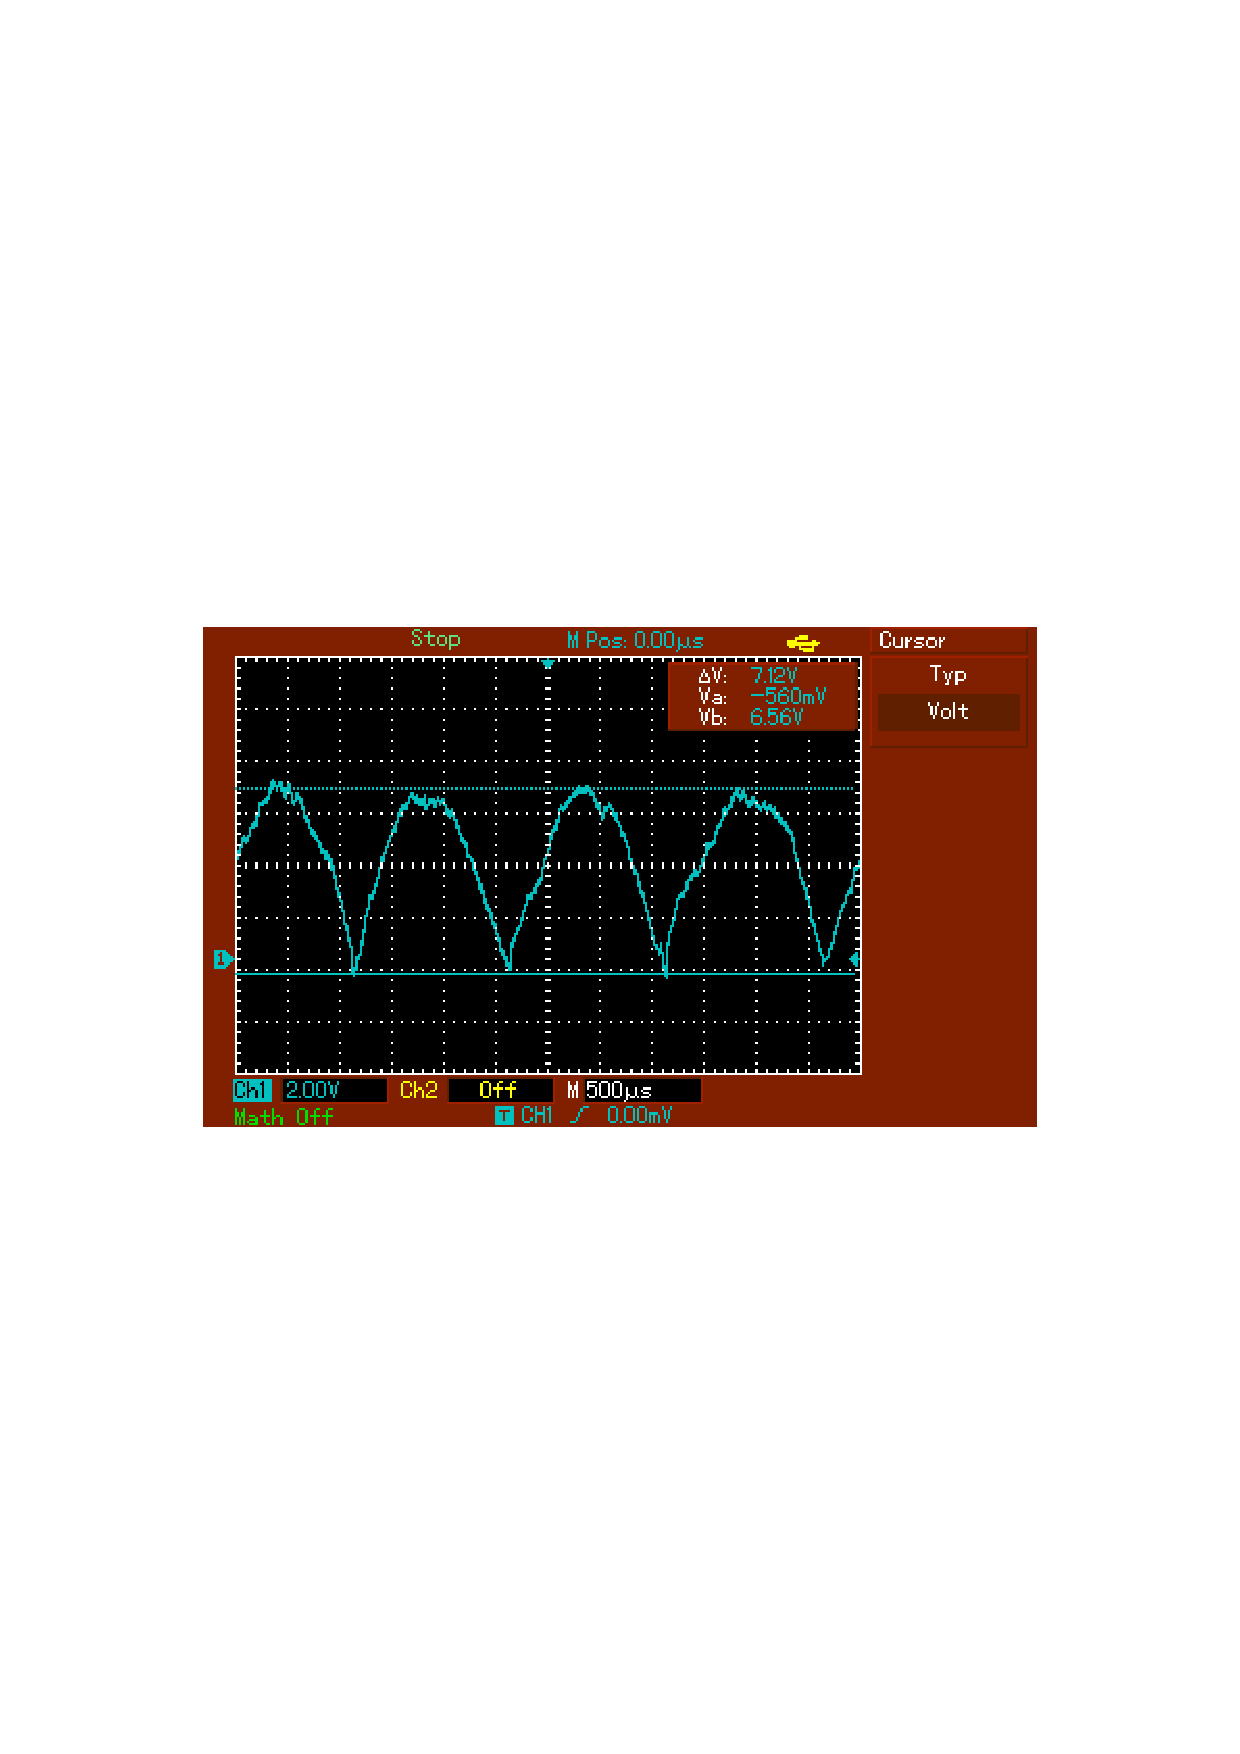
\includegraphics[height=5cm]{content/abbildungen/mit/240.pdf}
      \caption{Spannung bei $\phi = 240°$ mit Rauschen.}
  \end{subfigure}
\hfill 
  \begin{subfigure}{0.48\textwidth}
      \centering
      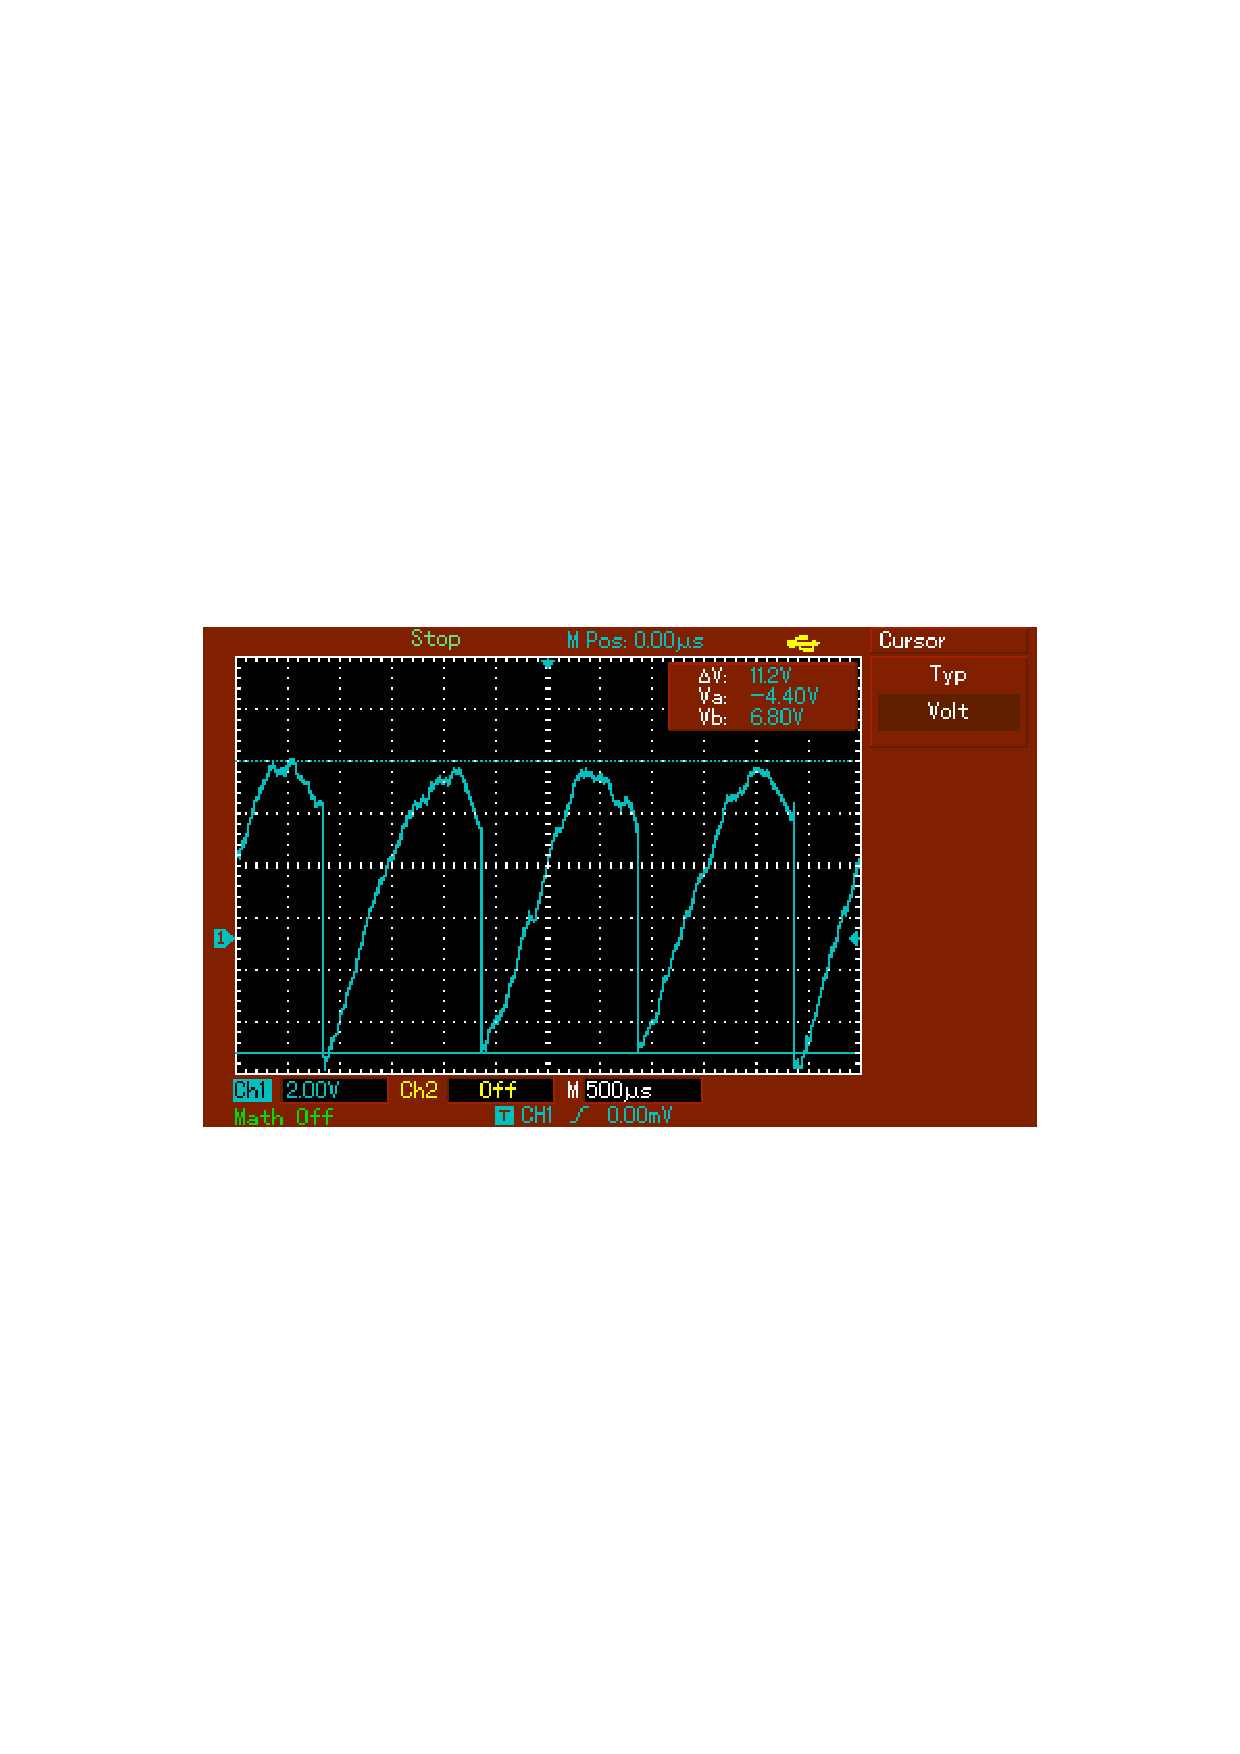
\includegraphics[height=5cm]{content/abbildungen/mit/300.pdf}
      \caption{Spannung bei $\phi = 300°$ mit Rauschen.}
  \end{subfigure}
\hfill 
  \begin{subfigure}{0.48\textwidth}
      \centering
      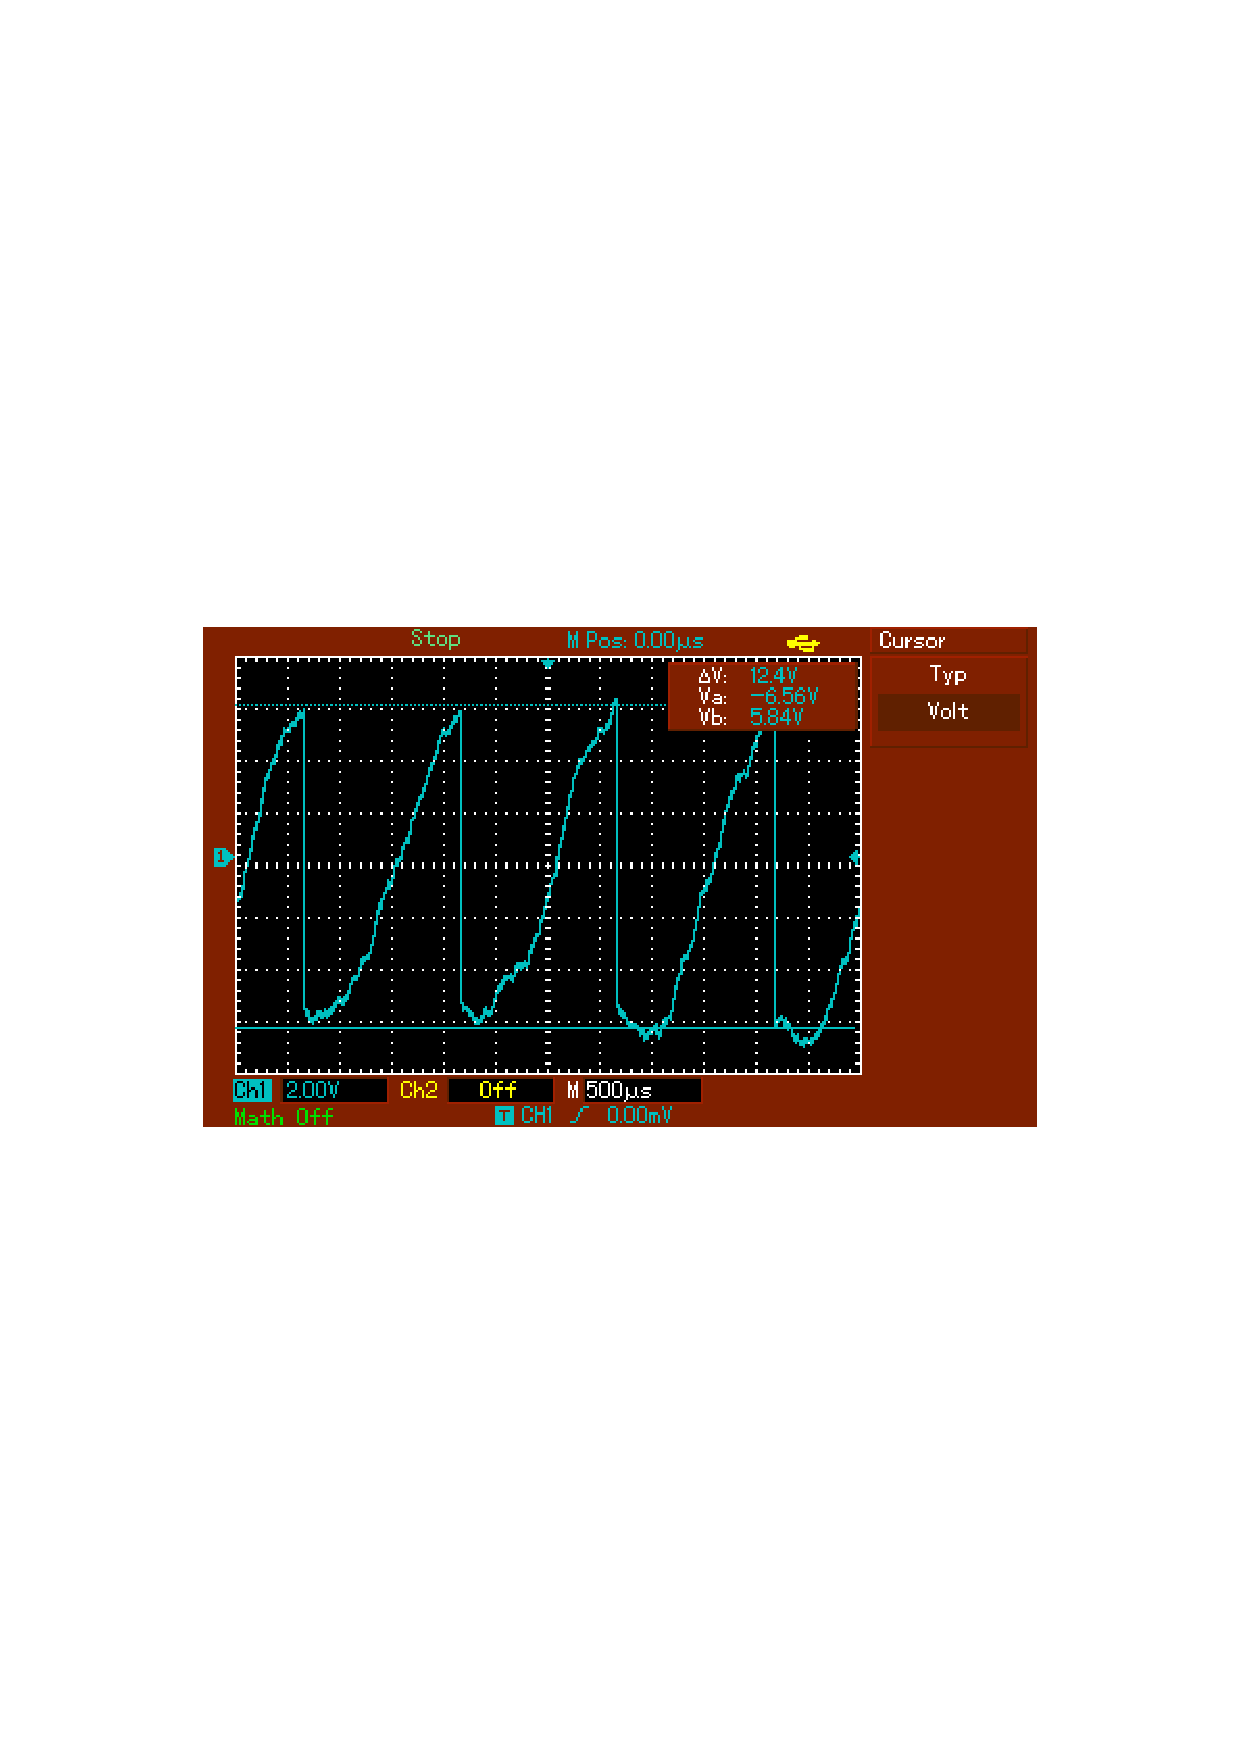
\includegraphics[height=5cm]{content/abbildungen/mit/360.pdf}
      \caption{Spannung bei $\phi = 360°$ mit Rauschen.}
  \end{subfigure}
\caption{Die Spannungen bei verschiedenen Phasenverschiebungen $\phi$ mit Noise Generator.}
\end{figure}

\begin{table} \label{tab:data_ohne_mit}
  \centering
  \caption{Die aufgenommenen Messergebnisse. Die Spannung in Abhängigkeit von der Phasenverschiebung $\phi$, mit und ohne Noise Generator. } 
  \begin{tabular}{c c c}
    \toprule
    $\increment \phi /°$ & $U_\text{ohne Noise} [\si{\volt}]$ & $U_\text{mit Noise} [\si{\volt}]$ \\
    \midrule
    0    &   8.4   &  5.85  \\
    60   &   9.5   &  3.72  \\
    120  &   7.5   &  6.2   \\
    180  &   8.1   &  6.4   \\
    240  &   10.2  &  3.56  \\
    300  &   7.5   &  5.6   \\
    360  &   8     &  6.2   \\
    \bottomrule
  \end{tabular}
\end{table}

\begin{figure} \label{fig:versuch_1_cosinus}
  \begin{subfigure}{0.56\textwidth}
      \centering
      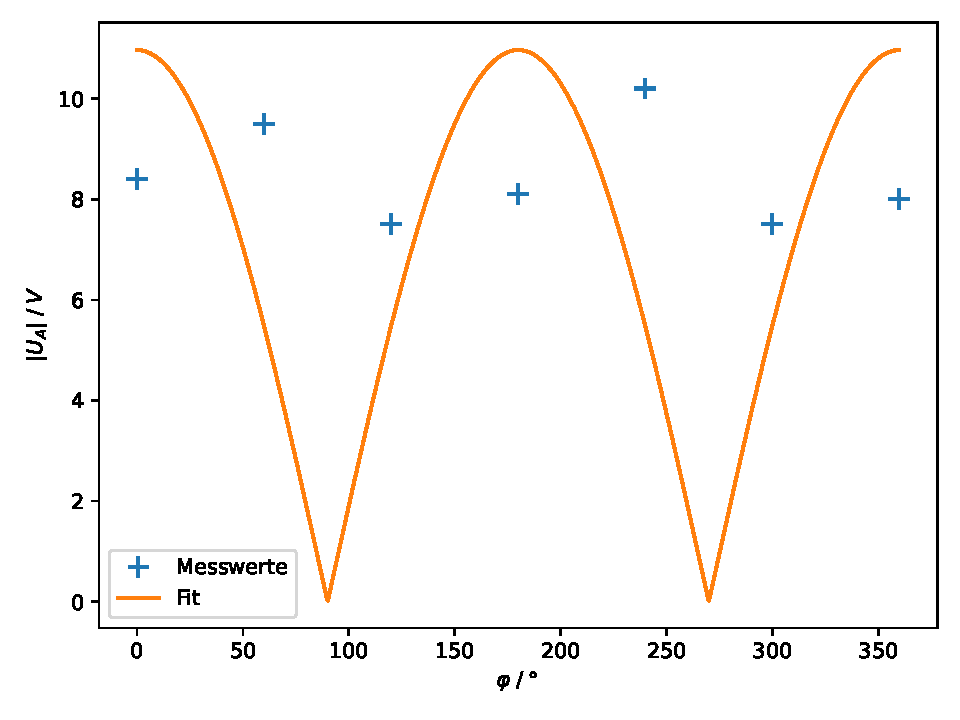
\includegraphics[height=4cm]{content/abbildungen/phasen_sonia.pdf}
      \caption{Die aufgenommenen Messwerte zum Versuchsdurchlauf ohne Noise Generator und die dazugehörige Ausgleichskurve.}
      \label{fig:ohne_noise}
  \end{subfigure}
\hfill
  \begin{subfigure}{0.40\textwidth}
      \centering
      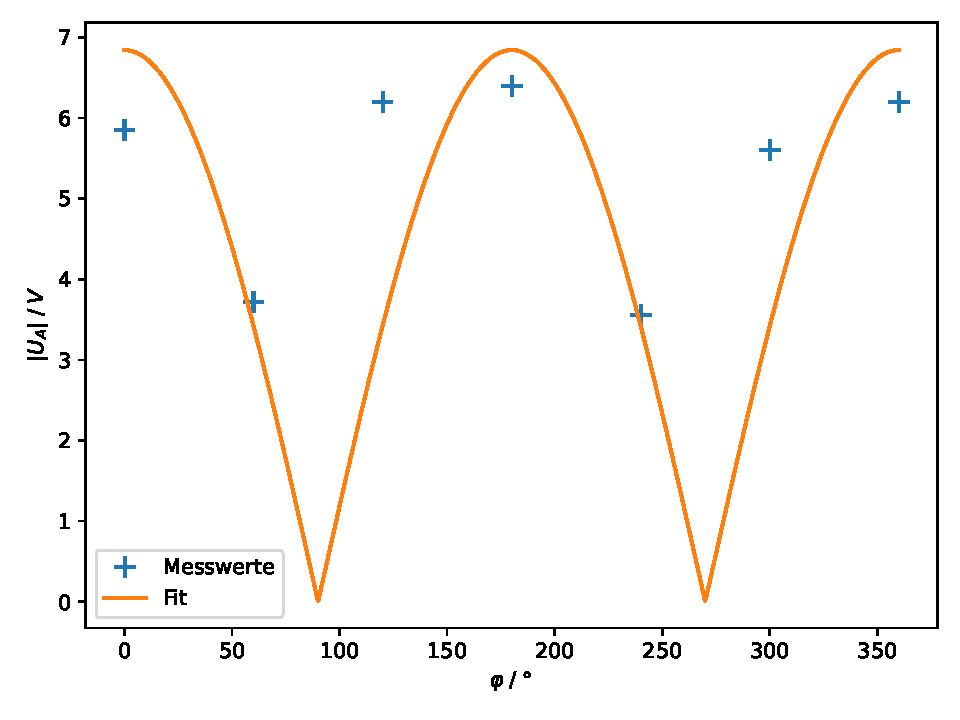
\includegraphics[height=3cm]{content/abbildungen/phasen_noise_sonia.pdf}
      \caption{Die aufgenommenen Messwerte zum Versuchsdurchlauf mit Noise Generator und die dazugehörige Ausgleichskurve.}
      \label{fig:mit_noise}
  \end{subfigure}
\end{figure}

\subsection{Untersuchung mit Photodiode}
\label{subsec:Photodiode}

Die aufgenommenen Messwerte sind in \autoref{tab:data_dioden} zu finden.
Mithilfe von ipython wird eine Ausgleichsrechnung nach der Form:
\begin{equation*}
  A = a \cdot \frac{1}{r} + b
\end{equation*}
durchgeführt.
Dabei ergeben sich folgende Parameter:
\begin{align*}
  a &= (84.59 \pm 1.85) \si{\volt\centi\metre}\\
  b &= (-1.07 \pm 0.16) \si{\volt}
\end{align*}

Die Messwerte und die dazugehörige Ausgleichskurve ist in \autoref{fig:plot3} zu sehen.
\begin{figure}
  \centering
  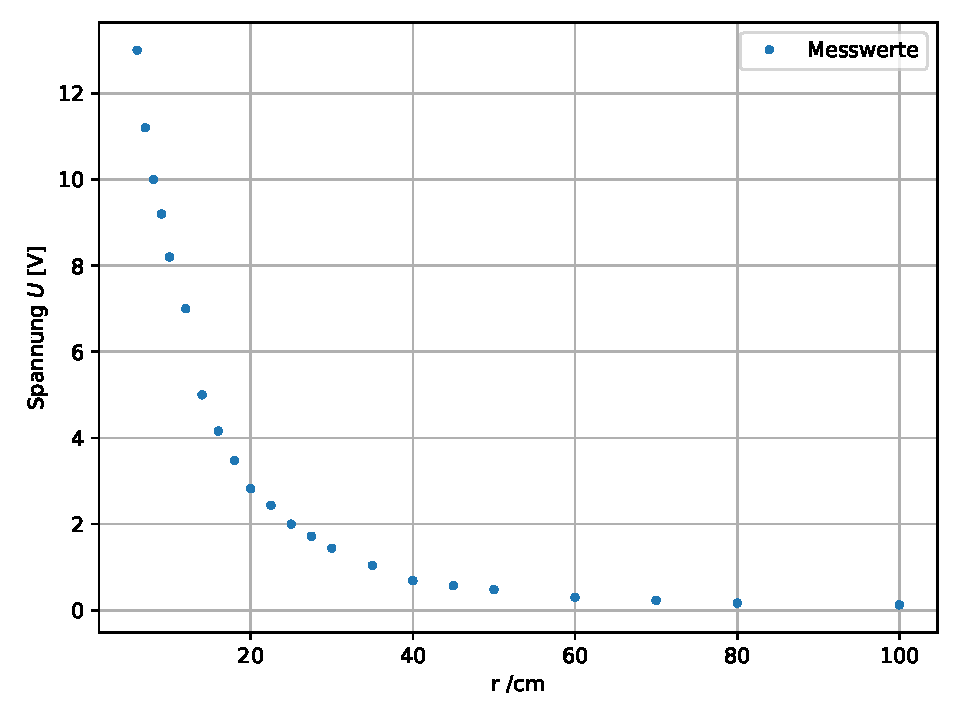
\includegraphics[width=\textwidth]{content/abbildungen/plot3.pdf}
  \caption{Die aufgenommenen Messwerte und die Ausgleichskurve.}
  \label{fig:plot3}
\end{figure}

\noindent
Da die Spannung und somit die Intensität mit $\frac{1}{r}$ abfällt, wurde ab einem Abstand von $\SI{40}{\centi\metre}$ eine Spannung im
$\si{\milli\volt}$ Bereich aufgenommen, eine genaue Nullspannung wurde nicht gemessen.
Der größte aufgenommene Abstand beträgt $\SI{100}{\centi\metre}$, die dazugehörige Spannung $\SI{126}{\milli\volt}$.

\begin{table}
  \centering
  \caption{Die aufgenommenen Messwerte. Die Spannung in Abhängigkeit vom Abstand $r$ zwischen den beiden Dioden. } 
  \label{tab:data_dioden}
  \begin{tabular}{c c}
    \toprule
    $r / \si{\centi\metre}$ & $A [\si{\volt}]$\\
    \midrule
    4.5    &   16.6  \\
  6.0    &   13.0  \\
  7.0    &   11.2  \\
  8.0    &   10.0  \\
  9.0    &   9.2   \\
  10.0   &   8.2   \\
  12.0   &   7.0   \\
  14.0   &   5.0   \\
  16.0   &   4.16  \\
  18.0   &   3.48  \\
  20.0   &   2.82  \\
  22.5   &   2.44  \\
  25.0   &   2.0   \\
  27.5   &   1.72  \\
  30.0   &   1.44  \\
  35.0   &   1.04  \\
  40.0   &   0.69  \\
  45.0   &   0.57  \\
  50.0   &   0.480  \\
  60.0   &   0.300  \\
  70.0   &   0.228  \\
  80.0   &   0.168  \\
  100.0  &   0.126  \\
    \bottomrule
  \end{tabular}
\end{table}
